\documentclass[a4paper]{ltxdoc}
\usepackage[british]{babel}
\usepackage[utf8]{inputenc}
\usepackage[T1]{fontenc}
\usepackage{newtxtext}
\usepackage[lmargin=4.5cm,rmargin=2cm,bottom=4cm,top=2cm]{geometry}
%\usepackage{array,booktabs,tabularx,longtable}
\usepackage[final]{listings}
\usepackage[onehalfspacing]{setspace}
%\usepackage{xspace}
\usepackage[dvipsnames]{xcolor}
%\usepackage{hologo}
\usepackage[%
pdftitle={},
pdfauthor={},
urlcolor=blue,%
linktocpage,%
colorlinks=true]{hyperref}
\usepackage{graphicx}

\providecommand*\pkg[1]{\textsf{#1}}
\makeatletter
\newcommand*\DescribeOption{%
\leavevmode%
\@bsphack%
\begingroup%
 \MakePrivateLetters%
 \Describe@Option%
}%
\newcommand*\Describe@Option[1]{%
 \endgroup%
\marginpar{%
 \raggedleft%
 \PrintDescribeEnv{#1}%
}%
\SpecialOptionIndex{#1}%
\@esphack%
\ignorespaces%
}%
\newcommand*\SpecialOptionIndex[1]{%
\@bsphack%
\index{%
 #1\actualchar{\protect\ttfamily#1} (option)\encapchar usage%
}%
\index{%
 options:\levelchar#1\actualchar{\protect\ttfamily#1}%
 \encapchar usage%
}%
\@esphack%
}%
\makeatother


\begin{document}
\author{Stefan Strecker (eic@emisa-journal.org) \and Martin Sievers (\ldots)}
\title{A \LaTeX{} class for preparing manuscripts for submissions to the OA  journal ‘Enterprise Modelling and Information Systems Architectures – An International Journal’ (EMISA)}
\maketitle
%\begin{abstract}
%\noindent XXX
%\end{abstract}




\section{Introduction}
Enterprise Modelling and Information Systems Architectures --~An International Journal (EMISA) is a publisher-independent, peer-reviewed scholarly open access journal (\url{http://emisa-journal.org}). 
EMISA is published by the German Informatics Society (GI) and is a publication of its Special Interest Group (SIG) on Modelling Business Information Systems (SIG MoBIS) and its SIG on Design Methods for Information Systems (SIG EMISA). SIG~MoBIS sponsored the development of the \pkg{EMISA} \LaTeX\ package currently maintained by Stefan Strecker, Editor-in-Chief of EMISA (eic@emisa-journal.org) and Martin Sievers (...).

The EMISA \LaTeX{} document class is provided for preparing manuscripts for submission to EMISA, and for preparing accepted submissions for publication as well as for typesetting the final publication by the editorial office. Articles in EMISA are published online at \url{http://emisa-journal.org} (in the Portable Document Format or PDF format).
The EMISA editorial office is run (alongside many other tasks and projects) by the two Editors-in-Chief assisted by three doctoral students. Editorial work at EMISA is best described as a volunteer effort for the scientific community.
Please assist us by preparing your manuscript following the instructions and guidelines described in this document: Your work will be published quicker with less (typographical) glitches and will have a professional appearance.





\section{Installation}
The EMISA \LaTeX\ package consists of the EMISA \LaTeX\ class \texttt{emisa.cls}, the BibLaTeX bibliography style \texttt{emisa.bbx} and the BibLaTeX control file \texttt{emisa.cbx}. 
The package also includes the present instructions and guidelines for authors on formatting the source files of the manuscript to achieve a pleasing and typographically consistent visual appearance of the reviewed as well as the published document.
Note that the package will (soon) be available from the \textsc{Comprehensive \TeX\ Archive Network} (CTAN, \url{https://ctan.org}) and should then be available for installation through the respective \TeX{} distribution’s package installer. In the meantime, a manual installation is required. For a manual installation, run \verb|pdflatex emisa.ins| and \verb|pdflatex emisa.dtx| twice, and copy the resulting files to the same folder / directory in which the source files for the manuscript will be maintained. 





\section{Instructions and guidelines}
This document provides instructions and guidelines for authors for manuscript preparation for EMISA. 
It covers all major aspects of scholarly writing (e.\,g.\ citations, references, figures, tables, source code and pseudocode listings).
Follow the instructions and guidelines in the present document to set up your files, to type in your text, to format figures, tables, source code listings and algorithms, and to obtain a consistent appearance in accordance with the journal's style specifications. 

It is recommended to use these instructions as a checklist before submitting your manuscript to the journal's online submission system at \url{http://emisa-journal.org}.
Note that these instructions are \emph{not} intended as a general introduction to \LaTeX2e{} and corresponding tools (see, for example, \url{https://www.ctan.org/tex-archive/info/lshort/english/} for ‘The not so Short Introduction to LaTeX’). 

%% XXX The following must be moved to the author instructions prepared using the ltxdoc package.



%
%%• The Reference Guide describing SVMono features with regards to their functionality.
%%Tip: Use it as a reference if you need to alter or enhance the default settings of the SVMono document class and/or the templates.
%
%%The documentation in the Springer SVMono tool package is not intended to be a general introduction to LATEX2ε or TEX. For this we refer you to [1–3].
%%Should we refer in this tool package to standard tools or packages that are not installed on your system, please consult the Comprehensive TEX Archive Network (CTAN) at [4–6].














\section{Preliminary remarks}
The \pkg{EMISA} document class is derived from the standard \LaTeX{} article class, and produces a customised two-column layout with bibliographic information about the manuscript in a multi-line page header (including the name of the journal, volume and issue number, year, title as well as author names) on A4-sized paper.
%
The \pkg{EMISA} class builds on a number of standard \LaTeX{} packages available in distributions such as \TeX{}Live and Mik\TeX{}. It is highly recommended to install the \emph{full} set of packages for the used distribution to make the required packages available to the \pkg{EMISA} class. Alternatively, missing packages may be installed on-the-fly.


The list of required packages for using the \pkg{EMISA} class is rather comprehensive (see \verb|emisa.cls|) but the class implementation has taken care to use only packages commonly included in \TeX\ distributions such as \TeX{}Live and Mik\TeX{}. Among the packages required by the \pkg{EMISA} class are \pkg{geometry}, \pkg{newtxtext}, \pkg{newtxmath}, \pkg{newtxtt}, \pkg{ntheorem}, \pkg{amsthm}, \pkg{booktabs}, \pkg{tabularx}, XXX.


The production process at the EMISA editorial office is based entirely on \LaTeX{}, and runs pdf\LaTeX{} and \verb|biber| to produce the final proof and publication of an article.  
The \pkg{biblatex} package is used to typeset citations and references in conjunction with the \verb|biber| tool. Make sure to use \verb|biber| rather than \verb|bibtex| to process the bibliography file(s).
The production tool chain at the editorial office requires that all text files of an article are provided in \emph{UTF-8 file encoding}\DescribeOption{UTF-8}, and that all line-drawing figures are submitted as vector graphics (\emph{not} bitmap graphics) in PDF format, and that all other (non-schematic) figures are submitted in PDF, JPEG or PNG format.   
 







\section{Class Options}
\DescribeOption{british} British English is the language of choice for publishing in EMISA. The class option ‘british’ must be used with the \pkg{EMISA} class to obtain the correct hyphenation for British English (as provided by the \pkg{babel} package). Example: \verb|\documentclass[british]{emisa}|.

\DescribeOption{referee, review} By default, a final version of the manuscript is typeset for online publication including the names and affiliations of authors. For reviewing purposes, the names and affiliations of the authors are omitted using the document option ‘referee’ or ‘review’ to allow for the anonymous (i.\,e.\ double blind) peer-review process of the EMISA journal. Example: \verb|\documentclass[british,referee]{emisa}|.






\section{Author information}
\DescribeMacro{\author}\DescribeMacro{\address}%
Each author is added using the macro \cs{author}\marg{author name} followed by the corresponding address \cs{address}\marg{author's address (line 1)\textbackslash\textbackslash\ \ldots (line 2)\textbackslash\textbackslash\ \ldots}. If you have multiple authors with the same address, please use \cs{address}\marg{author's address} only for the first one of those and \cs{address}\oarg{letter of address}\marg{} for all others.

\DescribeMacro{\author*}There has to be one corresponding author stated by \cs{author*}\marg{author's name}\marg{email address}.




\section{Title, subtitle, abstract, and keywords}
\DescribeMacro{\title}\DescribeMacro{\subtitle}%
The mandatory title and optional subtitle of a manuscript are typeset using \cs{title}\marg{title} and \cs{subtitle}\marg{subtitle}. 
%\pkg{EMISA} defines a \cs{title}\marg{title} and \cs{subtitle}\marg{subtitle} command for typesetting the manuscript title and subtitle. 
\DescribeMacro{\abstract}%
The abstract of the manuscript is typeset using \cs{abstract}\marg{abstract}. 
%Each manuscript should provide an abstract of about 200 words
\DescribeMacro{\keywords}%
Keywords describing the manuscript are typeset using \cs{keywords}\marg{keywords} and concatenated using \cs{and}. For example, \verb|\keywords{keyword1 \and keyword2}|. At least three keywords should be provided.



\section{Additional information on the first (title) page}
\DescribeMacro{\acknowledgments}%
Acknowledgements, for example, of collaborators, funding agencies etc.\ may be added using \cs{acknowledgements}\marg{acknowledgements}. The acknowledgements are typset in a footnote on the first page following the corresponding author’s email address.

\DescribeMacro{\authornote}%
Additional information for reviewers and readers may be added in a footnote on the titlepage using \cs{authornote}\marg{author note}. This is typically used for stating earlier publications (e.\,g.\ in conference proceedings) on which the present manuscript is based.



\section{Regular text}
A few conventional rules apply to writing regular text:
% for publication in the EMISA journal.

\begin{itemize}

\item Manuscripts should \emph{not} make use of outdated \LaTeX{} commands such as \verb|\em| but rather use the \LaTeX2e\ commands (e.g.\ \verb|\emph|, \verb|\texttt|). 


\item Do \emph{not} make use of bold face (\cs{textbf} or \cs{bf}). Use \cs{emph} instead to typeset an important word in italics!

\item Always use \verb|~| to connect before \cs{ref}\marg{label}, i.\,e.,\ \verb|Sec.~\ref{label}| rather than the problematic: \verb|Sec. \ref{label}|.

\item Do \emph{not} write abbreviations such as \verb|e.g.| but use the macros provided by the \pkg{EMISA} class (see below). Add punctuation when necessary, for example, write \verb|, \ie,| to achive the correct punctuation for ‘id est’ (i.\,e.) rather than \verb|, i.e.,| which introduces two problems: A missing spacing after the first full stop and a wrong spacing after the second full stop.



\item Follow the journal's style specification with respect to predefined text styles:

	\begin{itemize}
	\item Use \textsc{smallcaps} for names of open-source projects, products and companies etc, e.\,g.,\ \verb|\textsc{eclipse}| to produce \textsc{eclipse}.
	\item Use \texttt{non-proportional font} for language concepts, meta types, meta classes etc., e.\,g.,\ \verb|\texttt{AbstractGoalType}| to produce \texttt{AbstractGoalType}. 
	\item Use the \textsf{sans-serif font face} for type-level concepts etc., e.\,g.,\ \verb|\textsf{Goal}| to produce \textsf{Goal}.
	\end{itemize}

\end{itemize}







\section{Abbreviations and initialisms}
\DescribeMacro{\eg}\DescribeMacro{\ie}\DescribeMacro{\cf}\DescribeMacro{\etal}%
To achieve consistent typesetting of common abbreviations, macros are predefined by the \pkg{EMISA} class. These macros should consistently being used instead of writing the plain version. For example use \verb|\eg| rather than ‘\verb|e.g.|’. The macros take care of spacing within and after the abbreviations. The list of predefined abbrevations includes: %\cs{eg} \cs{ie} \cs{ea}

\begin{itemize}
\item \cs{eg} for e.\,g.
\item \cs{ie} for i.\,e.
\item \cs{cf} for cf.
\item \cs{etal} for et~al.
\end{itemize}


\DescribeMacro{\OMG}\DescribeMacro{\BPM}\DescribeMacro{\BPMN}\DescribeMacro{\UML}%
In addition to common abbreviations, further initialisms are provided by the class for convenience and for a consistent visual appearance. Note that the class uses \textsc{smallcaps} for typesetting initialisms following Brinkhurst XXX. The list of predefined initialisms includes:

\begin{itemize}
\item \cs{OMG} to obtain \textsc{omg} (Object Managment Group).
\item \cs{BPM} to obtain \textsc{bpm} (Business Process Management).
\item \cs{BPMN} to obtain \textsc{bpmn} (Business Process Model and Notation).
\item \cs{UML} to obtain \textsc{uml} (Unified Modeling Language).
\end{itemize}





\section{Quotation marks}
\DescribeMacro{\enquote}%
It is highly recommended to use the \cs{enquote}\marg{quotation} command to produce correct quotation marks in British English. Note that the command can be nested and will produce correct primary and secondary quotation marks, for example \verb|\enquote{A quote \enquote{with in a quote}}|.
Alternatively, the correct Unicode characters can be used, i.\,e.,\ Unicode 2018 and Unicode 2019 for the primary quotation marks, and Unicode 201C as well as Unicode 201D for the secondary quotation marks.
% or \LaTeX{} command \verb|\lq| for the opening primary quotation mark, and Unicode 2019 or \LaTeX{} command \verb|\rq| for the closing primary quotation mark.   






\section{Citations and references section}
\DescribeMacro{\parencite}\DescribeMacro{\textcite}\DescribeMacro{\cite}%
The EMISA journal uses its own author-year citation style predefined for the \pkg{biblatex} package (\verb|emisa.cbx|), and its own style for formatting entries in the list of references (\verb|emisa.bbx|). Consult the  \pkg{biblatex} package documentation for an introduction to the citation commands.
 It is important to use the citation commands properly to follow the journal's style specifications:

\begin{itemize}
\item \cs{parencite} is used for citing in parentheses (usually at the end of a sentence). In most cases, page numbers should be provided. Example: \verb|... is known \parencite[5]{Knuth1986}| produces ‘\ldots\ is known (Knuth 1986, p.~5)’.

\item \cs{textcite} allows for using the cited work as a subject in the grammatical structure of a sentence. Example: \verb|\textcite{Knuth1986} states that ...| produces ‘Knuth (1986) states that \ldots’. Additionally, page numbers and further information can be provided, see the \pkg{biblatex} package documentation.

\item \cs{cite} is used for typesetting the citation without parentheses, and is typically used within parentheses. Example: \verb|(see \cite{Knuth1986})| produces ‘(see Knuth 1986)’. This variant is the least used and should be used with care.
\end{itemize}

The \pkg{biblatex} package provides numerous extensions to the Bib\TeX\ format with respect to entry types and entry fields in the bibliographic database (see Chap.~2 in the package documentation). Make sure to provide full bibliographic information on all references but do \emph{not} use entry fields uncommon to scholarly writing, e.\,g.,\ entry fields such as \verb|isbn| or \verb|issn|.






\section{Figures}
All line-drawings must be provided as vector graphics (\emph{not} bitmap graphics) in PDF format and all other (non-schematic) figures (e.\,g.\ screenshots) must be provided in PDF, JPEG or PNG format in a proper (high) resolution for the intended size of the rendered image.

 
\begin{figure}[htbp]
\begin{center}
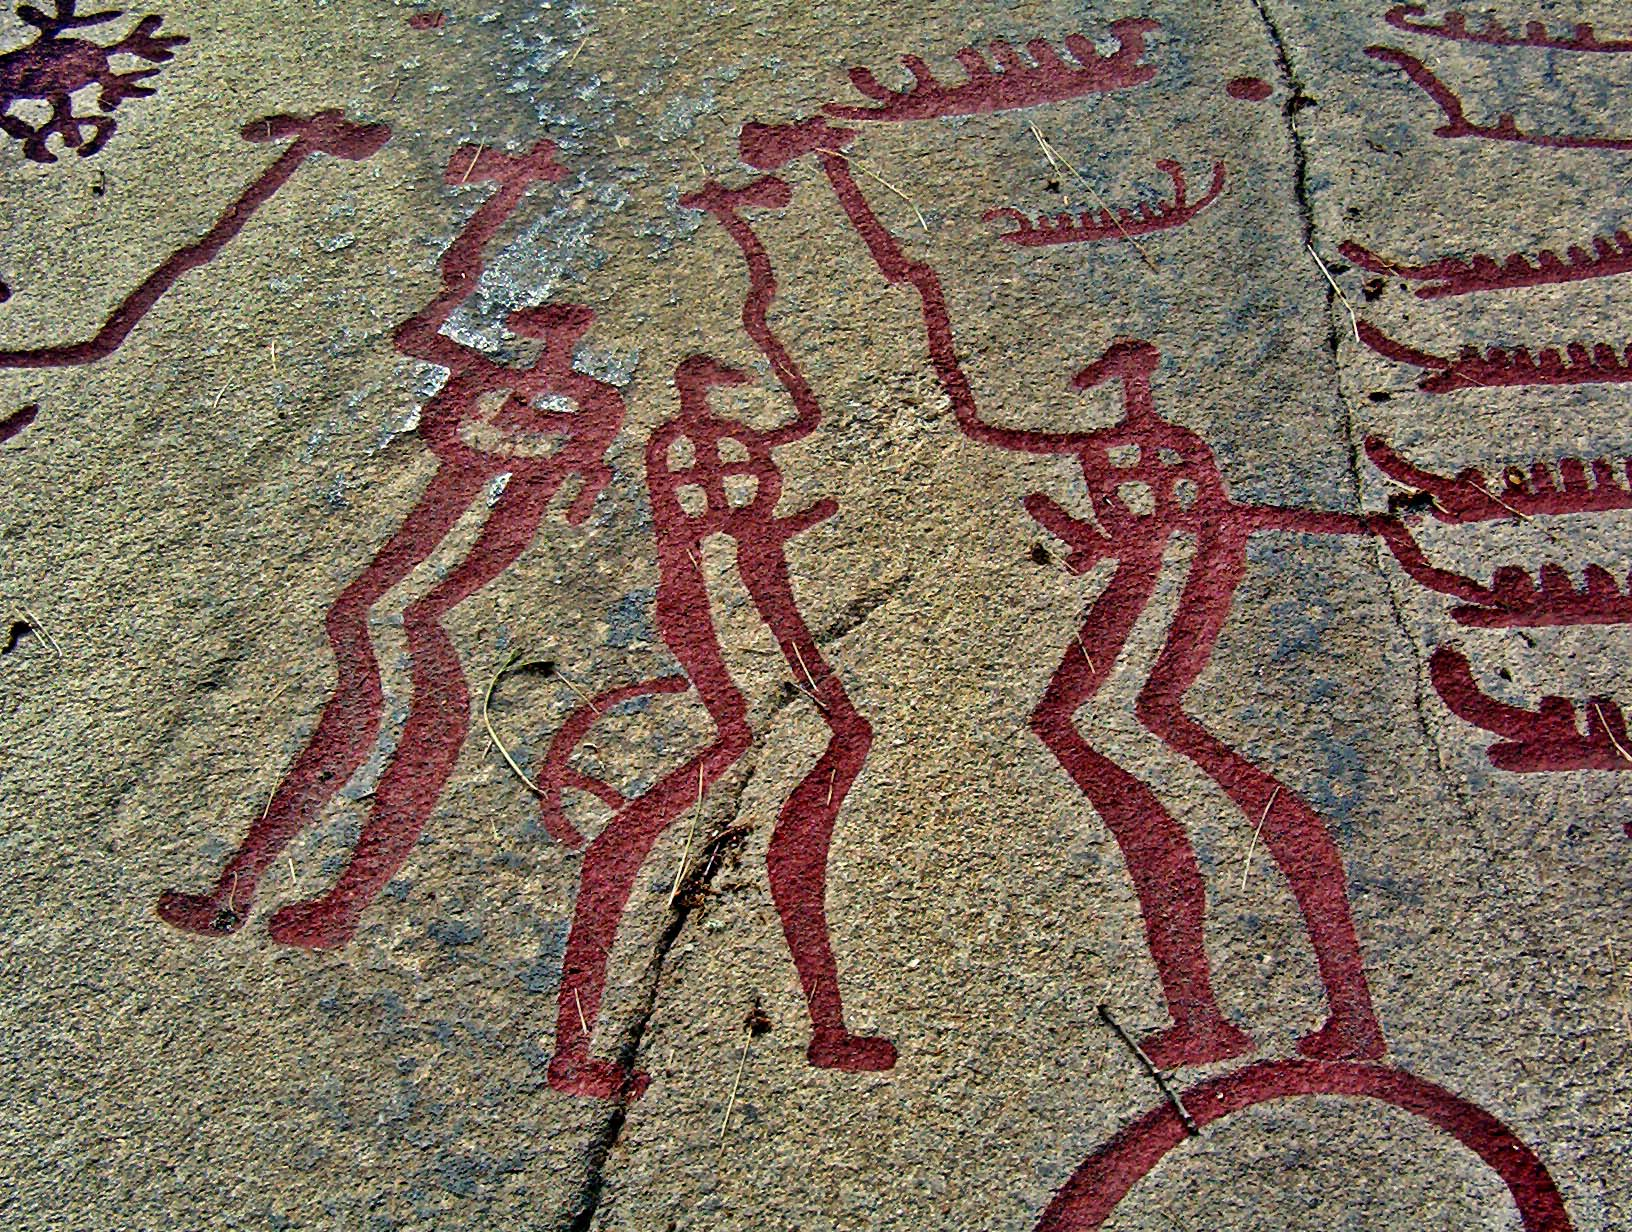
\includegraphics[width=0.5\textwidth]{bitmap}
\caption{Example. Non-schematic figure (bitmap graphic in JPEG format).}
\label{default}
\end{center}
\end{figure}



\begin{figure}[htbp]
\begin{center}
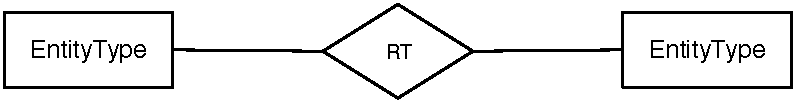
\includegraphics[width=0.5\textwidth]{vector}
\caption{Example. Line-drawing figure (vector graphic in PDF format).}
\label{default}
\end{center}
\end{figure}








\section{Tables}
\DescribeEnv{tabularx}






\section{Source code listings}
\DescribeEnv{sourcecode}\DescribeEnv{java}The \pkg{EMISA} class uses the \pkg{lstlistings} package for source code listings (see the package documentation for further information), and provides two customised \LaTeX\ environments: \cs{sourcecode} and \cs{java} XXX Hier kenne ich die Befehle zur Erstellung der Befehlsform nicht, \verb|\env| gibt es nicht XXX. The java environment should be used to format source code listings in the Java programming language, and the sourcecode environment should be used to format source code in any other programming language. Note that the source code in either case is typset verbatim, i.\,e.,\ the author must arrange the input \LaTeX\ source code according to the intended output. Also note that the two environments have been predefined to always produce a two-column listing positioned at the top of the page. An example illustrates the use of both environments:

XXX enter two examples here XXX




\section{Pseudocode and algorithms}
\DescribeEnv{algorithm}\DescribeEnv{algorithmcx}\pkg{EMISA} offers some environments for a comfortable integration of source code examples.




\end{document}
\endinput
